\chapter{Especificação: Projeto de Software}\label{cap:especificacao}

O presente capítulo apresenta os requisitos funcionais, não-funcionais e os diagramas de caso de uso para o projeto em questão.

\section{Requisitos funcionais}

Nesta seção serão apresentados os requisitos funcionais do aplicativo móvel.

\begin{description}
  \item[RF1] O aplicativo móvel deverá ser executado em um \textit{smartphone} ou \textit{tablet} com sistema operacional Android.
  %\item[RF2]  O aplicativo móvel deverá utilizar a Internet para seu correto funcionamento.
  %\subitem RF2.1 A conexão com a Internet deverá ser estabelecida de qualquer forma dentre as possíveis existentes, como uso de rede de dados 3G/4G ou WiFi.
  \item[RF2] O aplicativo móvel deverá coletar as coordenadas do dispositivo no qual está sendo executado.
  \item[RF3] O aplicativo móvel deverá apresentar ao usuário uma tela com as opções para acompanhamento de ônibus.
  \item[RF4] O aplicativo móvel deverá oferecer um recurso para que o usuário submeta \textit{feedbacks} sobre uma determinada linha de ônibus.
  \subitem RF4.1 Os \textit{feedbacks} deverão estar pré-definidos no aplicativo.
  \subitem RF4.2 Os \textit{feedbacks} devem conter informações relevantes sobre um determinado ônibus, como por exemplo, se o mesmo está lotado, se atrasou, ou se houve algum acidente no seu percurso.
  \item[RF5] O aplicativo móvel deverá armazenar as informações sobre uma determinada linha de ônibus.
  \subitem RF5.1 As informações deverão ficar armazenadas por, no máximo, 10 minutos.
  \subitem RF5.2 As informações podem ser provenientes do próprio usuário/dispositivo móvel ou de outros usuários/dispositivos móveis.
  \item[RF6] O aplicativo móvel deverá procurar por usuários/dispositivos próximos que estejam utilizando o aplicativo.
  \subitem RF6.1 Os dispositivos móveis devem estar com Wi-Fi ligado e executando o aplicativo móvel.
  \item[RF7] O aplicativo móvel deverá encaminhar suas informações armazenadas para quaisquer outros dispositivos móveis (\textit{smartphones} ou \textit{tablets}) encontrados.
  \subitem RF7.1 Os dispositivos móveis devem estar com Wi-Fi ligado e executando o aplicativo móvel.
  \item[RF8] O aplicativo móvel deverá oferecer ao usuário um recurso para mostrar um mapa informando a posição de um ônibus.
\end{description}

\section{Requisitos não-funcionais}

Nesta seção serão apresentados os requisitos não-funcionais do aplicativo móvel.

\begin{description}
  \item[RNF1] O aplicativo móvel deverá executar sobre o sistema operacional Android versão 4.1 (Jelly Bean), no mínimo.
  \item[RNF2]  O aplicativo móvel deverá utilizar a tecnologia Wi-Fi para seu correto funcionamento.
  \item[RNF3] O aplicativo móvel deverá utilizar uma arquitetura de rede descentralizada, integrando conceitos de DTN e P2P.
  \item[RNF4] O aplicativo móvel deverá ser desenvolvido na linguagem Java.
  \item[RNF5] O aplicativo móvel deverá ser desenvolvido utilizando o conjunto de ferramentas do Android SDK.
  \item[RNF6] O aplicativo móvel deverá ser desenvolvido utilizando o ambiente de desenvolvimento Android Studio.
\end{description}

\newpage

\section{Diagramas de Casos de Uso}

Esta seção apresenta o Diagrama de Casos de Uso para o aplicativo móvel a ser desenvolvido, bem como a descrição detalhada de cada caso. O diagrama pode ser observado na Figura \ref{fig:uc}.

\begin{figure}[h]
\begin{center}
    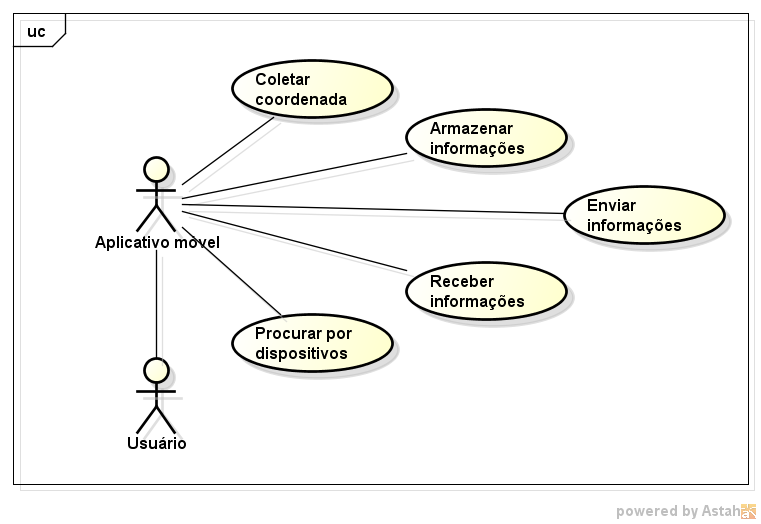
\includegraphics[width=1\columnwidth]{../figs/uc_tcc.png}
    \caption{Diagrama de Casos de Uso.}Fonte: Autoria própria.%\cite{sujatha}
    \label{fig:uc}
\end{center}
\end{figure}
%%%%%%%%%%%%%%%%%%%%%%%%%%%%%%%%%%%%%%%%%%%%%%%%%%%%%%%%%%%%%%%%%%%%%%%%%
\subsection{Coletar coordenada }

\noindent Nome: Coletar coordenada\\
Ator principal:Aplicativo móvel\\
Ator de bastidor: N/A\\
Descrição: quando se desejar conhecer a localização em que se encontra o dispositivo móvel, o GPS embutido no \textit{smartphone} será acionado para que as coordenadas sejam coletadas. \\\\\\\\
\textbf{Pré-condições:}
	\begin{itemize}
		\item O dispositivo móvel possui um sistema de GPS.
	\end{itemize}
\textbf{Pós-condições:}
	\begin{itemize}
		\item O GPS retorna a localização em que se encontra o dispositivo.
	\end{itemize}	
\textbf{Fluxo Básico:}
	\begin{enumerate}
		\item O Aplicativo móvel coleta a localização atual do dispositivo móvel, através do GPS integrado.
		\item As coordenadas obtidas pelo GPS são armazenadas na memória do \textit{smartphone}.
	\end{enumerate}	
\textbf{Fluxo Alternativo:}
	\begin{itemize}
		\item O Aplicativo móvel não consegue acionar o dispositivo de GPS: uma mensagem de erro é apresentada na tela do aparelho.
		\item O GPS é acionado, mas não é possível obter as coordenadas em que se encontra o dispositivo: uma mensagem de erro é apresentada na tela do aparelho.
		\item Não há espaço suficiente para armazenar as novas coordenadas obtidas do GPS: uma mensagem de erro é apresentada na tela do aparelho.
	\end{itemize}
\textbf{Regras de Negócio:}	nenhuma.
%%%%%%%%%%%%%%%%%%%%%%%%%%%%%%%%%%%%%%%%%%%%%%%%%%%%%%%%%%%%%%%%%%%%%%%%%
\subsection{Armazenar informações }

\noindent Nome: Armazenar informações\\
Ator principal:	Aplicativo móvel\\
Ator de bastidor: Usuário\\
Descrição: este caso de uso ocorre quando o usuário submete alguma informação referente à algum ônibus, quando as coordenadas são coletadas ou quando informações são recebidas de outros dispositivos.\\\\
\textbf{Pré-condições:}
	\begin{itemize}
		\item Necessário haver informações para armazenamento, sejam elas inseridas pelo próprio usuário, coletadas pelo GPS integrado ou recebidas de outros dispositivos.
	\end{itemize}
\textbf{Pós-condições:}
	\begin{itemize}
		\item Informação é armazenada na memória do dispositivo, por 10 minutos.
	\end{itemize}	
\textbf{Fluxo Básico:}
	\begin{enumerate}
		\item Após o Usuário submeter alguma informação, o aplicativo móvel armazena-a em memória por 10 minutos.
	\end{enumerate}	
\textbf{Fluxo Alternativo I:}
	\begin{enumerate}
		\item Informações são recebidas de outros dispositivos.
		\item Essas informações são armazenadas em memória por 10 minutos.
	\end{enumerate}
\textbf{Fluxo Alternativo II:}
	\begin{enumerate}
		\item A coordenada do dispositivo foi coletada.
		\item Armazena a coordenada em memória, por 10 minutos.
	\end{enumerate}
\textbf{Regras de Negócio:}	nenhuma.

%%%%%%%%%%%%%%%%%%%%%%%%%%%%%%%%%%%%%%%%%%%%%%%%%%%%%%%%%%%%%%%%%%%%%%%%%
\subsection{Enviar informações }

\noindent Nome: Enviar informações\\
Ator principal:	Aplicativo móvel\\
Ator de bastidor: Usuário\\
Descrição: este caso de uso ocorre quando há informações armazenadas no dispositivo, prontas para serem enviadas.\\\\
\textbf{Pré-condições:}
	\begin{itemize}
		\item Necessário haver informações para envio, sejam elas inseridas pelo próprio usuário, coletadas pelo GPS integrado ou recebidas de outros dispositivos. 
		\item Outros dispositivos móveis nas proximidades devem estar conectados e executando a aplicação.
	\end{itemize}
\textbf{Pós-condições:}
	\begin{itemize}
		\item Informações são enviadas para outros dispositivos móveis próximos que estejam conectados.
	\end{itemize}	
\textbf{Fluxo Básico:}
	\begin{enumerate}
		\item O Usuário decide notificar demais usuários sobre alguma informação relevante.
		\item O Usuário seleciona a informação no menu com opções pré-definidas.
		\item O Usuário confirma determinada informação para o ônibus em específico.
		\item O Aplicativo móvel envia a informação para quaisquer outros dispositivos móveis próximos que estejam conectados.
		\item A informação fica armazenada em memória por 10 minutos.
	\end{enumerate}	
\textbf{Fluxo Alternativo I:}
	\begin{itemize}
		\item Informações são recebidas de outros dispositivos móveis.
		\item As informações são repassadas para demais dispositivos móveis próximos que estejam conectados.
		\item Essas informações ficam armazenadas em memória por 10 minutos.
	\end{itemize}
\textbf{Fluxo Alternativo II:}
	\begin{enumerate}
		\item A coordenada do dispositivo foi coletada.
		\item A coordenada é repassada para demais dispositivos móveis próximos que estejam conectados.
		\item A coordenada fica armazenada em memória por 10 minutos.
	\end{enumerate}
\textbf{Regras de Negócio:}	nenhuma.

%%%%%%%%%%%%%%%%%%%%%%%%%%%%%%%%%%%%%%%%%%%%%%%%%%%%%%%%%%%%%%%%%%%%%%%%%
\subsection{Receber informações }

\noindent Nome: Receber informações\\
Ator principal:	Aplicativo móvel\\
Ator de bastidor: N/A\\
Descrição: este caso de uso ocorre quando o aplicativo móvel recebe informações/mensagens de outros dispositivos.\\\\
\textbf{Pré-condições:}
	\begin{itemize}
		\item As mensagens recebidas devem estar construídas de acordo com um protocolo pré-configurado no dispositivo.
		\end{itemize}
\textbf{Pós-condições:}
	\begin{itemize}
		\item As informações/mensagens são armazenadas na memória por 10 minutos.
	\end{itemize}	
\textbf{Fluxo Básico:}
	\begin{enumerate}
		\item O aplicativo móvel recebe uma informação/mensagem de outro dispositivo móvel.
		\item O aplicativo móvel verifica se reconhece o padrão da mensagem recebida.
		\item O aplicativo móvel armazena a nova mensagem na memória de mensagens recebidas (para consulta local).
		\item O aplicativo móvel armazena a nova mensagem na memória de mensagens a enviar (para propagar a mensagem a outros dispositivos).
	\end{enumerate}	
\textbf{Fluxo Alternativo:}
	\begin{itemize}
		\item A mensagem recebida não possui os padrões esperados e é automaticamente descartada.
		\item A memória destinada a alocação de mensagens recebidas está cheia: uma mensagem de notificação é mostrada na tela do dispositivo.
	\end{itemize}
\textbf{Regras de Negócio:}	nenhuma.

%%%%%%%%%%%%%%%%%%%%%%%%%%%%%%%%%%%%%%%%%%%%%%%%%%%%%%%%%%%%%%%%%%%%%%%%%
\subsection{Procurar por dispositivos }

\noindent Nome: Procurar por dispositivos\\
Ator principal:	Aplicativo móvel\\
Ator de bastidor: Usuário\\
Descrição: este caso de uso ocorre periodicamente durante a execução do aplicativo móvel.\\\\
\textbf{Pré-condições:}
	\begin{itemize}
		\item O aplicativo móvel deve estar executando.
		\item O Wi-Fi no dispositivo móvel deve estar ligado.
	\end{itemize}
\textbf{Pós-condições:}
	\begin{itemize}
		\item Uma conexão é estabelecida com outros dispositivos móveis que estejam próximos e executado o aplicativo.
	\end{itemize}	
\textbf{Fluxo Básico:}
	\begin{enumerate}
		\item O Usuário liga a conexão Wi-Fi no dispositivo móvel.
		\item O Usuário inicia o Aplicativo móvel.
		\item O Aplicativo móvel procura por outros dispositivos móveis nas proximidades.
		\item Se um dispositivo é encontrado, inclui o mesmo na lista de dispositivos encontrados e estabelece conexão.
		\item O Aplicativo móvel aguarda dois minutos.
		\item Realiza nova busca, retornando ao passo 3.
	\end{enumerate}	
\textbf{Fluxo Alternativo:}
	\begin{itemize}
		\item O usuário pressiona o botão para procurar por dispositivos imediatamente.
		\item Vai para o passo 3 do Fluxo Básico.
	\end{itemize}
\textbf{Regras de Negócio:}	nenhuma.

